% Figure 4: Temporal Stability (2010 → 2020)
% Requires data from paper 7 (temporal stability analysis)

\begin{figure*}[t]
\centering

% Panel A: Tract retention rates
\begin{subfigure}[b]{0.32\textwidth}
\centering
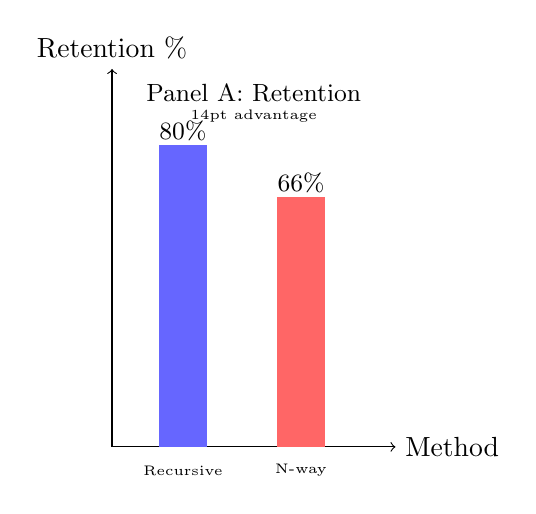
\begin{tikzpicture}[scale=0.6]
% Bar chart comparing methods
\draw[->] (0,0) -- (0,8) node[above] {Retention \%};
\draw[->] (0,0) -- (6,0) node[right] {Method};

% Recursive bisection bar
\fill[blue!60] (1,0) rectangle (2,6.4);
\node at (1.5,-0.5) {\tiny Recursive};
\node at (1.5,6.7) {\small 80\%};

% N-way bar
\fill[red!60] (3.5,0) rectangle (4.5,5.28);
\node at (4,-0.5) {\tiny N-way};
\node at (4,5.6) {\small 66\%};

% Labels
\node at (3,7.5) {\small Panel A: Retention};
\node at (3,7) {\tiny 14pt advantage};
\end{tikzpicture}
\caption{Census tract retention}
\end{subfigure}
\hfill
% Panel B: Variance decomposition
\begin{subfigure}[b]{0.32\textwidth}
\centering
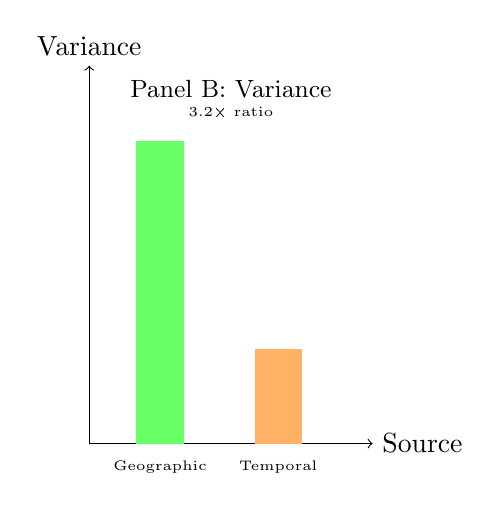
\begin{tikzpicture}[scale=0.6]
% Bar chart of variance sources
\draw[->] (0,0) -- (0,8) node[above] {Variance};
\draw[->] (0,0) -- (6,0) node[right] {Source};

% Geographic variance
\fill[green!60] (1,0) rectangle (2,6.4);
\node at (1.5,-0.5) {\tiny Geographic};

% Temporal variance
\fill[orange!60] (3.5,0) rectangle (4.5,2);
\node at (4,-0.5) {\tiny Temporal};

% Ratio label
\node at (3,7.5) {\small Panel B: Variance};
\node at (3,7) {\tiny 3.2× ratio};
\end{tikzpicture}
\caption{Geographic vs. temporal}
\end{subfigure}
\hfill
% Panel C: Boundary overlay
\begin{subfigure}[b]{0.32\textwidth}
\centering
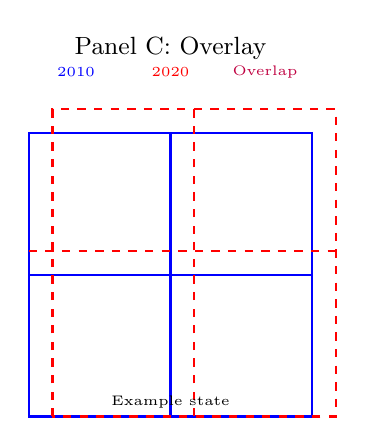
\begin{tikzpicture}[scale=0.6]
% Placeholder map overlay
\draw[blue, thick] (0,0) rectangle (6,6);
\draw[blue, thick] (3,0) -- (3,6);
\draw[blue, thick] (0,3) -- (6,3);

\draw[red, thick, dashed] (0.5,0) rectangle (6.5,6.5);
\draw[red, thick, dashed] (3.5,0) -- (3.5,6.5);
\draw[red, thick, dashed] (0,3.5) -- (6.5,3.5);

% Legend
\node[blue] at (1,7.3) {\tiny 2010};
\node[red] at (3,7.3) {\tiny 2020};
\node[purple] at (5,7.3) {\tiny Overlap};

\node at (3,7.8) {\small Panel C: Overlay};
\node at (3,0.3) {\tiny Example state};
\end{tikzpicture}
\caption{District boundary changes}
\end{subfigure}

\caption{\textbf{Temporal stability across census cycles.} (A) Recursive bisection maintains 80\% census tract retention from 2010 to 2020 redistricting, outperforming n-way partitioning (66\%) by 14 percentage points. The hierarchical structure creates geographic scaffolding that persists across demographic change. (B) Variance decomposition reveals that differences between geographic regions (e.g., urban vs. rural) exceed temporal changes by 3.2×, indicating districts reflect durable spatial structure rather than decade-specific population artifacts. (C) District boundary overlay (example state) shows 2010 boundaries (blue) and 2020 boundaries (red); purple overlap illustrates high spatial consistency despite population shifts.}
\label{fig:temporal}
\end{figure*}

% NOTE: This is a placeholder template. Actual figure requires:
% - Tract retention data from paper 7 temporal stability analysis
% - Variance decomposition statistics
% - Geographic boundary shapefiles for 2010 and 2020
% - Map overlay generation (recommend Georgia or Alabama for clear example)
% - Python/R script: research/00+synthesis-metapaper/scripts/generate_figure4.py
